%%%%%%%%%%%%%%%%%%%%%%%%%%%%%%%%%%%%%%%%%%%%%%
%Lab report writeup based on template by Derek Hildreth
%%%%%%%%%%%%%%%%%%%%%%%%%%%%%%%%%%%%%%%%%%%%%%

%\documentclass[aps,letterpape,10pt]{revtex4}
\documentclass[aps,letterpaper,10pt]{article}
%\documentclass{article}

\usepackage{graphicx} % For images
\usepackage{float}    % For tables and other floats
\usepackage{verbatim} % For comments and other
\usepackage{amsmath}  % For math
\usepackage{amssymb}  % For more math
\usepackage{fullpage} % Set margins and place page numbers at bottom center
\usepackage{subfig}   % For subfigures
\usepackage[usenames,dvipsnames]{color} % For colors and names
\usepackage{fancyhdr} %headers
\usepackage{listings} %for code
\usepackage{color} %to color code
\usepackage{wrapfig} % for inline images

%Color and code setup
\definecolor{dkgreen}{rgb}{0,0.6,0}
\definecolor{gray}{rgb}{0.5,0.5,0.5}
\definecolor{mauve}{rgb}{0.58,0,0.82}
\definecolor{codebg}{rgb}{.95,.95,.98}

\lstset{ %
	language=Python, 
	tabsize=4, 
	numbers=left,
	numberstyle=\footnotesize,
	backgroundcolor=\color{codebg},
	breaklines=true,
	breakatwhitespace=true,
	basicstyle=\small,
	numberstyle=\tiny\color{black},
	showstringspaces=false,
	keywordstyle=\color{blue}, 
	stringstyle=\color{dkgreen},
	commentstyle=\color{gray},
	frame=single,
	title = \texttt{\lstname}
	}

%%%%%%%%%%%%

%HEADER FORMATING%%%%%%%%%%%%%
\pagestyle{fancy}
\headheight 10pt
\setlength{\headsep}{20pt}
\lhead{MPHY 396 - Prof. Suzuki\\ Homework 8}
\rhead{A. Athanassiadis\\Due 2/22/2012}
%%%%%%%%%%%%%%%%%%%%%%%%

%Custom Definitions%%%%%%%%%%%%%%%
\newcommand{\ttt}{\texttt}
%%%%%%%%%%%%%%%%%%%%%%%%

\begin{document}
\section{Problem 1}
\textbf{What is the benefit of polar coordinates in the Hough transform?}\\

If the free parameters defining the Hough space axes came from the Cartesian coordinate equation $y=kx+q$, then a very large Hough space image would be required to represent a single point.  The set of lines that pass through a point $(x,y)$ includes many very steep $(|k|>>1)$ lines with large intercepts $(|q|>>1)$. As a result, the Hough space image would need to be orders of magnitude larger than the input image, which is often times impractical.  Moreover, it would be impossible to represent a vertical line in such a Hough space because it would require $k\rightarrow\infty.$  Additionally, it would be impossible to represent any lines with $k<1$ in the discrete Hough space.  Thus, choosing the Cartesian parameters would greatly limit the effectiveness of the Hough transform.

The polar formulation that is traditionally used circumvents these limitations because it can parametrize a line by an angle $\theta$ with the $x$ axis and its perpendicular distance $r$ to the origin.  The polar parametric form of the line allows lines to be represented by finite coefficients in Hough space:
\begin{eqnarray*}
\theta & : & 0\rightarrow 2\pi \\
r & : & 0\rightarrow\max(H_{im},W_{im})
\end{eqnarray*}
where $H_{im}$ and $W_{im}$ are the image height and width respectively.  Additionally, these variables can be discretized and still retain a good deal of representative power.  These features make the polar form a natural coordinate system to employ when searching for lines in images using the Hough transform.

\section{Problem 2}
\textbf{Explain why the lines generated by the Hough transform are infinite in length.}\\

The Hough transform specifies a point by the set of lines that pass through it using polar coordinates $r$ and $\theta$.  A point $(x,y)$ in real space is thus represented by the curve $\{(r,\theta)_H|\, r = x\cos(\theta) + y\sin(\theta)\}$ in Hough space. A line segment in real space is consequently represented by the intersection of many Hough transform curves corresponding to the different points lying on the line segment.

If the Hough space intersection point, $(r^\star,\theta^\star)_H$ is the only information used to reconstruct the input image, then it corresponds to an infinite line because there is no information encoded in the Hough space point that specifies end conditions for the line segment in real space.  One thing to note is that based on the size of the Hough space image and on the values of other points in Hough space, it should be possible to reconstruct a line segment with specific length.  It is only when a single point (or small subset of the Hough space) $(r^\star,\theta^\star)_H$ is used that the reconstructed line loses all end point information.

\section{Problem 3}
\textbf{Develop and implement a Hough transform that detects circles.}
\begin{figure}[!h]
\centering
\subfloat[Original Image]{\label{fig:8-3a}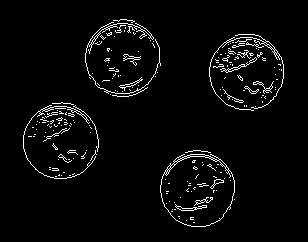
\includegraphics[width=.3\textwidth]{img_hough_circle.png}} \hfill
\subfloat[Hough Transformed Image]{\label{fig:8-3b}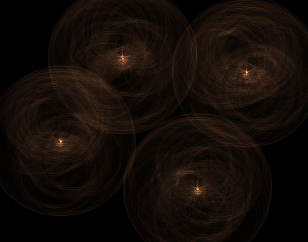
\includegraphics[width=.3\textwidth]{hough_t.png}} \hfill
\subfloat[Inverse Hough Transform Overlay]{\label{fig:8-3c}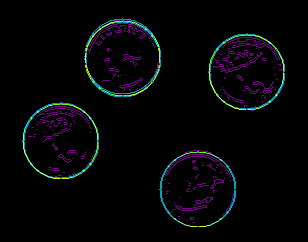
\includegraphics[width=.3\textwidth]{inverse_hough.png}}
\caption{Hough Transformations}
\label{fig:8-3}
\end{figure}

The Hough transform algorithm I implemented here was designed to find circular boundaries of radius $38$px, which was measured from the original image in Figure \ref{fig:8-3a}.  The coordinates in this Hough space are $(a,b)_H$, which correspond to the only unknown variables (the circle centers) in the equation $$(x-a)^2+(y-b)^2=R^2.$$
Every point $(x,y)$ in the original image is mapped to the set of points $\{(a,b)_H |\, (x-a)^2+(y-b)^2=R^2\}$.  The Hough transformed image in Figure \ref{fig:8-3b} is the sum of the transformations of every point in the real space image.  The brightest points indicate the Hough space parameters that many real space points could correspond to.  Therefore, these bright sections reveal the centers of circles in the original image.  I manually thresholded the Hough transformed image and reconstructed circles around the remaining points.  The results are displayed in Figure \ref{fig:8-3c} and are overlayed with the original image.  The blue and green points are the reconstructed borders.  The purple points are the original image.  Because the free parameters that defined the Hough space axes were spatial coordinates of the center of circles, the inverse transformation simply required running the thresholded Hough transform image through the transformation algorithm.

\lstinputlisting{problem3.py}

\section{Appendix: Common Code}
The base code used for Problem 3 in this homework is contained in \ttt{circhough.py}.
\lstinputlisting{circhough.py}
\end{document} 